\documentclass[reprint,amsmath,amssymb,aps]{revtex4-2}

\usepackage{graphicx} % Include figure files
\usepackage{dcolumn} % Align table columns on decimal point
\usepackage{bm} % bold math
\usepackage{hyperref} % add hypertext capabilities
\usepackage[spanish,mexico]{babel}
\usepackage{float} %usar [H]
\usepackage{diagbox}
% \graphicspath{{imagenes/}} %Carpetas donde estaran las imagenes

\begin{document}

\preprint{APS/123-QED}

\title{Template-based Routing Generator}
\author{José de Jesús de la Rosa de la Rosa}
\email{a228835@alumnos.uaslp.mx}
\affiliation{Facultad de Ciencias, Universidad Autónoma de San Luis Potosí.}
\date{22 de junio de 2022}

\begin{abstract}

\end{abstract}

%\keywords{HOLA,JH,OK}

\maketitle 

\section{Introducción}

Durante años se han propuesto en la literatura técnicas de enrutamiento para la automatización del diseño de circuitos integrados (IC) digitales y analógicos. En ellas, ya se ha cubierto un amplio conjunto de restricciones geométricas para la la mejora de calidad del enrutamiento, pero también se han incluido progresivamente criterios relacionados con el rendimiento. Sin embargo, a medida que el diseño de circuitos mas complejos y de características particulares, como en los circuitos analógicos y de radiofrecuencia, avanzan hacia nuevos nodos tecnológicos, el creciente número de reglas y restricciones de diseño, la resistencia de cables, la congestión y el crecimiento de circuitos parasíticos entre cables, impulsan constantemente las técnicas de enrutamiento automático existentes y mantienen la presión sobre su mejora.

En la literatura se han propuesto técnicas de enrutamiento para la automatización del diseño de circuitos integrados analógicos y de radiofrecuencia (A/RF)~\cite{unutulmaz, martins}. En ellas, ya se ha cubierto un amplio conjunto de restricciones geométricas como sustitutos de la calidad del enrutamiento, pero también se han incluido progresivamente criterios relacionados con el rendimiento. Sin embargo, a medida que el diseño de circuitos A/RF avanza hacia nodos tecnológicos de integración avanzada, el creciente número de reglas ó restricciones de diseño, la resistencia de los cables, la congestión y el crecimiento parasitario entre cables desafían constantemente las técnicas de enrutamiento automático existentes y mantienen la presión sobre su mejora. Afortunadamente, los recientes avances en las capacidades de las estaciones de trabajo modernas permitieron el crecimiento de sofisticados procesos de enrutamiento, incluidos algunos asistidos por los últimos métodos de aprendizaje automático y profundo, que ofrecen soluciones sin precedentes para la automatización de esta tarea. Sin embargo, la correlación entre las estructuras parasíticas inducidas por el enrutamiento y el comportamiento funcional del circuito dista mucho de ser sencilla, también se han propuesto técnicas de síntesis computacionalmente intensivas con inclusión de parásitos y conscientes del diseño, en las que las técnicas de enrutamiento automático desempeñan un papel decisivo.\\

\section{Path-finding algorithm}

Una de las principales técnicas es el uso de generadores de enrutamiento basados en plantillas (TbRG, \textit{Template-based routing generators}). La plantilla actúa como una representación del diseño gráfico de la tecnología, generada por el conjunto y características de los dispositivos. Son especialmente útiles cuando se debe migrar un diseño validado previamente diseñado, es decir, un diseño heredado, a otros nodos de tecnología cercanos o se necesitan cambios en el diseño. Esta plantilla puede ser implementada como un grafo de pesos unitarios, conexo y no dirigido, donde se seleccionan un vértice origin y destino, y a través de diferentes algoritmos, encontrar el camino mas corto.

El algoritmo de Dijkstra, también llamado algoritmo de caminos mínimos, es un algoritmo para la determinación del camino más corto, dado un vértice origen, hacia el resto de los vértices en un grafo que tiene pesos en cada arista. La idea general en este algoritmo consiste en ir explorando todos los caminos más cortos que parten del vértice origen y que llevan a todos los demás vértices, cuando se obtiene el camino más corto desde el vértice origen hasta el resto de los vértices que componen el grafo, el algoritmo se detiene. Se trata de una especialización de la búsqueda de costo uniforme y, como tal, no funciona en grafos con aristas de coste negativo (al elegir siempre el nodo con distancia menor, pueden quedar excluidos de la búsqueda nodos que en próximas iteraciones bajarían el costo general del camino al pasar por una arista con costo negativo).

Existe una variante del algoritmo de Dijkstra, llamado algoritmo A*, el cual tiene como objetivo únicamente el camino más corto desde una fuente específica hasta un objetivo específico, y no el árbol de caminos más corto desde una fuente específica hasta todos los objetivos posibles. Para esto es es necesario el uso de una función heucarística. Para el algoritmo de Dijkstra, dado que se genera todo el árbol de la ruta más corta, cada nodo es un objetivo y no puede haber una heurística dirigida a un objetivo específico, obteniendo peor rendimiento que el algoritmo A* cuando la búsqueda del camino mas corto es solo entre dos nodos.

\begin{figure}[H]
 	\centering
 	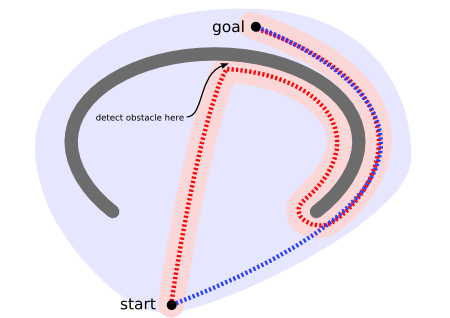
\includegraphics[width=0.48\textwidth]{concave1.png}
 	\caption{Algoritmo pathfinding.}
 	\label{concave1}
\end{figure}
 
\begin{figure}[H]
 	\centering
 	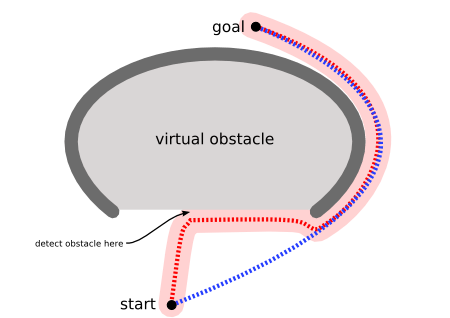
\includegraphics[width=0.48\textwidth]{concave2.png}
 	\caption{Algoritmo pathfinding.}
 	\label{concave2}
\end{figure}

El Algoritmo de Dijkstra funciona visitando los vértices del grafo empezando por el punto inicial del objeto. A continuación, examina repetidamente el vértice más cercano aún no examinado, añadiendo sus vértices al conjunto de vértices por examinar. Se expande hacia fuera desde el punto de partida hasta alcanzar la meta. Se garantiza que el Algoritmo de Dijkstra encuentra el camino más corto desde el punto de partida hasta la meta, siempre que ninguna de las aristas tenga un coste negativo. (Escribo "un camino más corto" porque a menudo hay múltiples caminos equivalentemente cortos). En el siguiente diagrama, el cuadrado rosa es el punto de partida, el cuadrado azul es la meta, y las áreas de color verde azulado muestran las áreas que el Algoritmo de Dijkstra escaneó. Las zonas cerceta más claras son las más alejadas del punto de partida y, por tanto, constituyen la "frontera" de la exploración:

\begin{figure}[H]
 	\centering
 	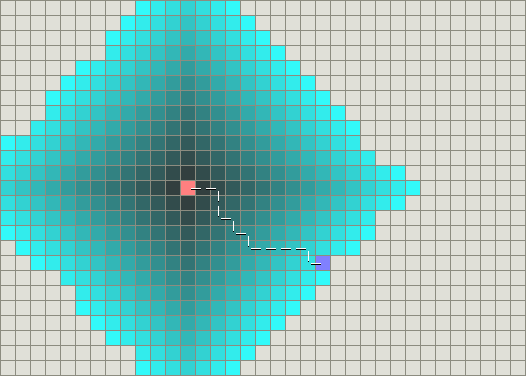
\includegraphics[width=0.48\textwidth]{dijkstra.png}
 	\caption{Algoritmo pathfinding.}
 	\label{dijkstra}
\end{figure}

The Greedy Best-First-Search algorithm works in a similar way, except that it has some estimate (called a heuristic) of how far from the goal any vertex is. Instead of selecting the vertex closest to the starting point, it selects the vertex closest to the goal. Greedy Best-First-Search is not guaranteed to find a shortest path. However, it runs much quicker than Dijkstra’s Algorithm because it uses the heuristic function to guide its way towards the goal very quickly. For example, if the goal is to the south of the starting position, Greedy Best-First-Search will tend to focus on paths that lead southwards. In the following diagram, yellow represents those nodes with a high heuristic value (high cost to get to the goal) and black represents nodes with a low heuristic value (low cost to get to the goal). It shows that Greedy Best-First-Search can find paths very quickly compared to Dijkstra’s Algorithm:

\begin{figure}[H]
 	\centering
 	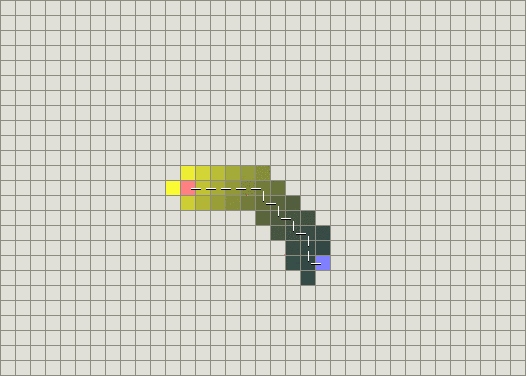
\includegraphics[width=0.48\textwidth]{greedy.png}
 	\caption{Algoritmo pathfinding.}
 	\label{a}
\end{figure}

Sin embargo, ambos ejemplos ilustran el caso más sencillo: cuando el mapa no tiene obstáculos y el camino más corto es realmente una línea recta. Consideremos el obstáculo cóncavo descrito en la sección anterior. El Algoritmo de Dijkstra es más difícil, pero se garantiza que encuentra el camino más corto:

\begin{figure}[H]
 	\centering
 	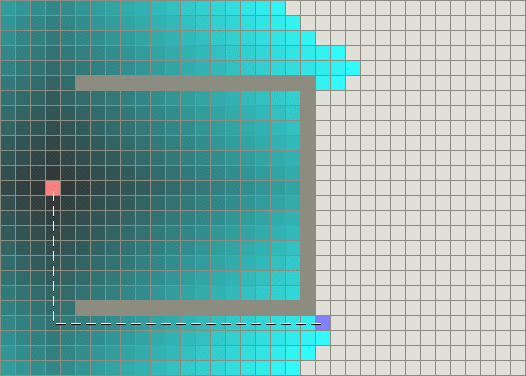
\includegraphics[width=0.48\textwidth]{dijkstra-trap.png}
 	\caption{Algoritmo pathfinding.}
 	\label{dijkstra-trap}
\end{figure}
 
Greedy Best-First-Search on the other hand does less work but its path is clearly not as good. The trouble is that Greedy Best-First-Search is “greedy” and tries to move towards the goal even if it’s not the right path. Since it only considers the cost to get to the goal and ignores the cost of the path so far, it keeps going even if the path it’s on has become really long.
 
\begin{figure}[H]
 	\centering
 	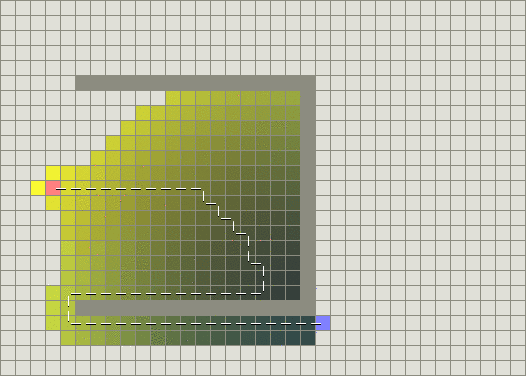
\includegraphics[width=0.48\textwidth]{greedy-trap.png}
 	\caption{Algoritmo pathfinding.}
 	\label{a-trap}
\end{figure}

¿No estaría bien combinar lo mejor de ambos? A* se desarrolló en 1968 para combinar enfoques heurísticos como el de Greedy Best-First-Search y enfoques formales como el Algoritmo de Dijsktra. Es algo inusual, ya que los enfoques heurísticos suelen ofrecer una forma aproximada de resolver problemas sin garantizar que se obtenga la mejor respuesta. Sin embargo, A* se construye sobre la heurística, y aunque la heurística en sí no le da una garantía, A* puede garantizar un camino más corto.

Me centraré en el algoritmo A*. A* es la opción más popular para la búsqueda de caminos, porque es bastante flexible y se puede utilizar en una amplia gama de contextos.

A* es como el Algoritmo de Dijkstra en el sentido de que puede utilizarse para encontrar el camino más corto. A* se parece al algoritmo Greedy Best-First-Search en que puede utilizar una heurística para guiarse. En el caso simple, es tan rápido como el algoritmo Greedy Best-First-Search:

\begin{figure}[H]
	\centering
	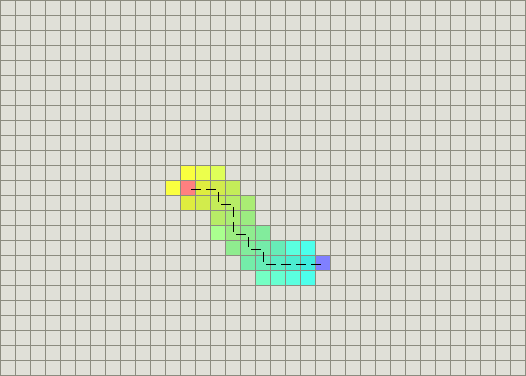
\includegraphics[width=0.48\textwidth]{a-star.png}
	\caption{Algoritmo pathfinding.}
	\label{a-trap}
\end{figure}

\begin{figure}[H]
	\centering
	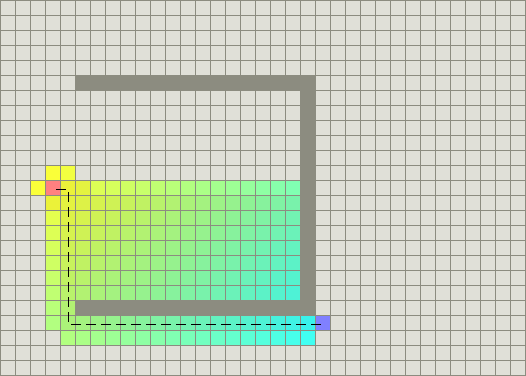
\includegraphics[width=0.48\textwidth]{a-star-trap.png}
	\caption{Algoritmo pathfinding.}
	\label{a-trap}
\end{figure}

El secreto de su éxito es que combina la información que utiliza el Algoritmo de Dijkstra (favoreciendo los vértices que están cerca del punto de partida) y la información que utiliza el Greedy Best-First-Search (favoreciendo los vértices que están cerca de la meta). En la terminología estándar utilizada al hablar de A*, g(n) representa el coste exacto del camino desde el punto de partida hasta cualquier vértice n, y h(n) representa el coste heurístico estimado desde el vértice n hasta la meta. En los diagramas anteriores, el amarillo (h) representa los vértices alejados de la meta y el verde azulado (g) representa los vértices alejados del punto de partida. A* equilibra ambos a medida que se desplaza desde el punto de partida hasta la meta. Cada vez que pasa por el bucle principal, examina el vértice n que tiene el valor más bajo f(n) = g(n) + h(n).

La capacidad de A* de variar su comportamiento en función de la heurística y las funciones de coste puede ser muy útil en un juego. El equilibrio entre velocidad y precisión puede aprovecharse para hacer el juego más rápido. Para la mayoría de los juegos, en realidad no necesitas el mejor camino entre dos puntos. Necesitas algo que esté cerca. Lo que necesitas puede depender de lo que está pasando en el juego, o de lo rápido que es el ordenador. Usar una función que garantiza que nunca sobreestima el coste significa que a veces lo subestimará bastante.

La heurística estándar para una cuadrícula cuadrada es la distancia Manhattan. Mira tu función de costes y encuentra el coste mínimo D para moverte de un espacio a otro adyacente. En el caso simple, puedes fijar D en 1. La heurística en una cuadrícula cuadrada donde se puede mover en 4 direcciones debe ser D veces la distancia de Manhattan:

función heurística(nodo) =
    dx = abs(nodo.x - meta.x)
    dy = abs(nodo.y - meta.y)
    return D * (dx + dy)

¿Cómo se elige D? Utiliza una escala que se ajuste a tu función de costes. Para los mejores caminos, y una heurística "admisible", establece D al menor coste entre cuadrados adyacentes. En ausencia de obstáculos, y en un terreno que tenga el mínimo coste de movimiento D, acercarse un paso a la meta debería aumentar g en D y disminuir h en D. Cuando sumas los dos, f (que se establece en g + h) permanecerá igual; eso es señal de que la heurística y las escalas de la función de coste coinciden. También puedes renunciar a caminos óptimos para hacer que A* corra más rápido aumentando D, o disminuyendo la relación entre los costes de arista más bajos y más altos.

\section{Implementación}

\section{Trabajo a futuro}

\section{Conclusiones}




\section{Conclusiones}
A pesar de las diferentes arquitecturas de memorias basadas en RRAM reportadas en la literatura, no ha sido reportada una celda que logre una implementación funcional debido los problemas derivados de la variabilidad de los dispositivos.
  
\bibliographystyle{unsrtnat}
\nocite{*}
\bibliography{citas}% Produces the bibliography via BibTeX.

\end{document}
